\section{Power}
\label{sec:power}
\textit{\hyperlink{schematic.8}{schematic}}

\subsection{Overview}
\label{sec:power-overview}

A barrel jack is used to feed a 12V input to the board which is then administered to a 10V output
linear regulator and two buck converters that output 5.6V and 3.6V. The buck converters in turn pass
their voltages on to several LDO voltage regulators for input to the various digital ICs on the
board. The benefit of chaining switching converters to linear regulators is greater energy
efficiency and better noise suppression than can be achieved by using either alone. An LED indicates
when power is administered to the board.

\subsection{Barrel Jack / Power Input}
\label{sec:power-input}

A ferrite bead pi filter is placed at the output of the barrel jack connection. The ferrite bead is
rated for $5.1A$, which is more than double the absolute max current draw of the radar. The barrel
connector is a switched jack, but we do not use a battery on this PCB so the 3rd pin is grounded.

\subsection{TPS5420D Buck Converter}
\label{sec:tps5420d}

\subsubsection{Description}
\label{sec:tps5420d-description}

The TPS5420D is an internally-compensated buck converter with a fixed switching frequency of
$500\si{kHz}$, whose block diagram is shown in Figure~\ref{fig:tps5420d-block}. The converter first
compares the divided voltage output with a $1.221V$ reference and uses an error amplifier to amplify
the difference. It then feeds that difference into a PWM comparator along with a sawtooth ramp
waveform. If the PWM comparator outputs a high voltage the switch is turned off, effectively
decreasing the duty cycle. Conversely, a low voltage saturates the transistor and increases the duty
cycle. This has the effect of converging the output voltage to its set point.

\begin{figure}[h]
        \centering
        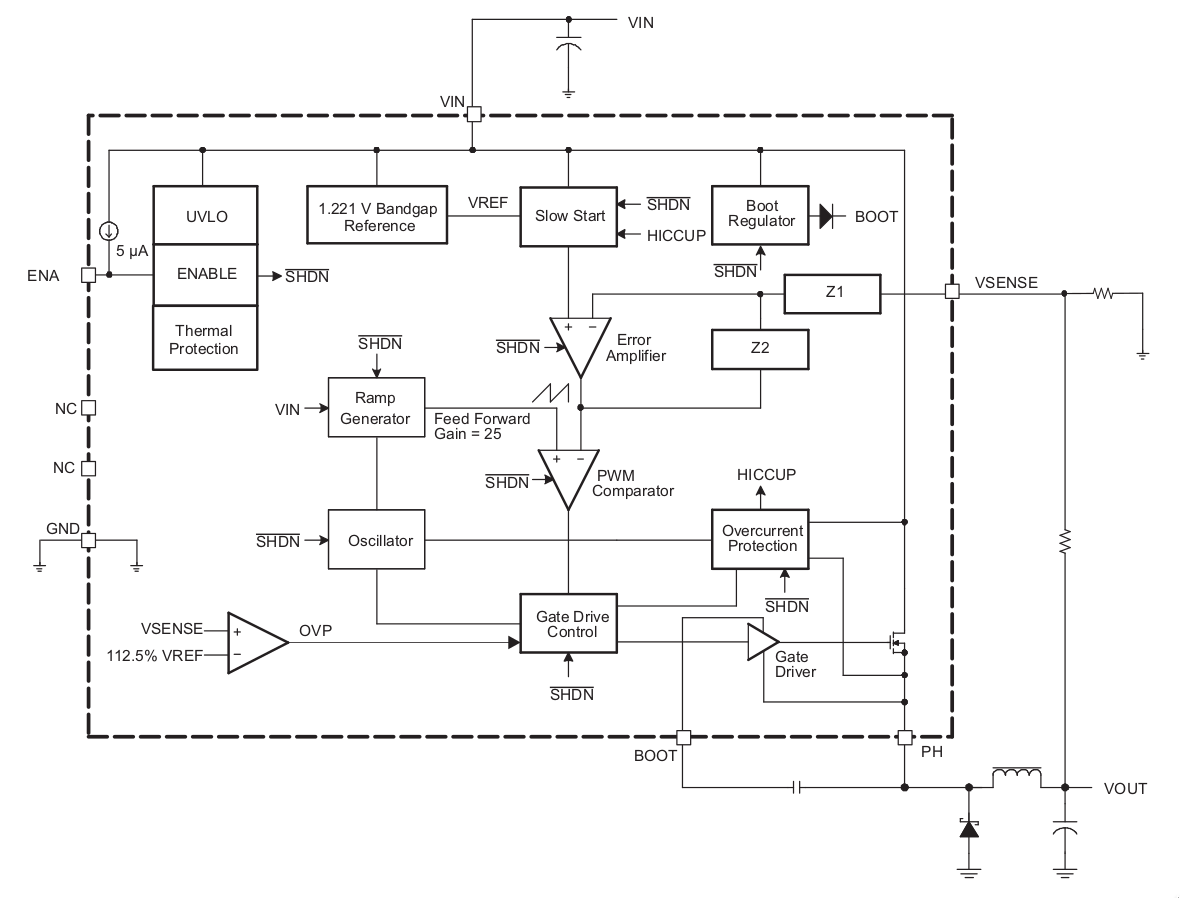
\includegraphics[width=0.9\textwidth]{data/tps5420d-block-diagram}
        \caption{TPS5420D Block Diagram}
        \label{fig:tps5420d-block}
\end{figure}

\subsubsection{Downstream Current Draw}
\label{sec:tps5420d-current}

\label{tab:buck-5.6-current}
\begin{tabularx}{\textwidth}{l c c X>{\raggedright\arraybackslash}X}
        \caption{The current draw of components downstream from the 5.6V buck converter. When
          minimum current draw is omitted from the datasheet I've assumed 0A.} \\
        \toprule
        \textbf{MFN} & \textbf{I\textsubscript{Q}} & \textbf{I\textsubscript{max}} & \textbf{Voltage
        Inputs} \\
        \midrule \endhead
        \hyperlink{sec:adl5802}{ADL5802} & $170\si{mA}$ & $300\si{mA}$ & 5V \\
        \hyperlink{sec:adf4158}{ADF4158} & $312.5\si{\mu A}$ & $5\si{mA}$ & 5V (VP) \\
        \hyperlink{sec:se5004l}{SE5004L} & $300\si{mA}$ & $800\si{mA}$ & 5V (VCC1, VCC2, VCC3) \\
        \midrule
        Total & $470\si{mA}$ & $1.105\si{A}$ & - \\
        \bottomrule
\end{tabularx}

\label{tab:buck-3.6-current}
\begin{tabularx}{\textwidth}{l c c X>{\raggedright\arraybackslash}X}
        \caption{Components downstream from the 3.6V buck converter.} \\
        \toprule
        \textbf{MFN} & \textbf{I\textsubscript{Q}} & \textbf{I\textsubscript{max}} & \textbf{Voltage
        Inputs} \\
        \midrule \endhead
        \hyperlink{sec:kt2520k}{KT2520K}  & - & $2\si{mA}$ & 1.8V \\
        \hyperlink{sec:nc7s04}{NC7S04} & $1\si{\mu A}$ & $12.5\si{mA}$ & 3.3V \\
        \hyperlink{sec:nb3n551}{NB3N551} & - & $40\si{mA}$ & 3.3V \\
        \midrule
        \hyperlink{sec:xc7a15t-ftg256}{XC7A15T-FTG256} & $97\si{mA}$ & $277\si{mA}$ & 1V (VCCINT,
        VCCBRAM) \\
        XC7A15T-FTG256 & $22\si{mA}$ & $87\si{mA}$ & 1.8V (VCCADC, VCCAUX) \\
        XC7A15T-FTG256 & $1\si{mA}$ & $201\si{mA}$ & 3.3V (VCC0) \\
        \hyperlink{sec:w25q32jv}{W25Q32JV} & $10\si{\mu A}$ & $25\si{mA}$ & 3.3V \\
        \midrule
        \hyperlink{sec:ft2232h}{FT2232H} & $510\si{\mu A}$ & $280\si{mA}$ & 3.3V (VPHY, VPLL, VCORE,
        VCCIO) \\
        \hyperlink{sec:93lc46b}{93LC46B} & - & $2\si{mA}$ & 3.3V \\
        \midrule
        \hyperlink{sec:ltc2292}{LTC2292} & $5\si{mA}$ & $95\si{mA}$ & 3.3V (OVDD), 3V (VDD) \\
        \midrule
        \hyperlink{sec:ada4940-2}{ADA4940-2} & $4.2\si{mA}$ & $5.52\si{mA}$ & 3.3V \\
        \midrule
        \hyperlink{sec:adf4158}{ADF4158} & - & $32\si{mA}$ & 3.3V (AVDD, DVDD) \\
        \midrule
        \hyperlink{sec:hmc431lp4}{HMC431LP4} & $19\si{mA}$ & $27\si{mA}$ & 3V \\
        \midrule
        \hyperlink{sec:trf37a73}{TRF37A73} & $250\si{\mu A}$ & $130\si{mA}$ & 3V \\
        \hyperlink{sec:sky65404}{SKY65404} & $20\si{mA}$ & $36\si{mA}$ & 3V (VENABLE, VCC) \\
        \midrule
        Total & $169\si{mA}$ & $1.252\si{A}$ & - \\
        \bottomrule
\end{tabularx}

\subsubsection{Pinout}
\label{sec:tps5420d-pinout}

\fixme{What is the point of BOOT?}
\label{tab:tps5420d-pinout}
\begin{tabularx}{\textwidth}{l X>{\raggedright\arraybackslash}X}
        \caption{TPS5420D pinout.} \\
        \toprule
        \textbf{Pin} & \textbf{Description} \\
        \midrule \endhead
        BOOT & \\
        VSENSE & Feedback voltage for the regulator. This compares the divided output with a 1.221V
        reference. \\
        ENA & Enable pin. This can be left floating to enable the device. \\
        VIN & Input supply voltage. \\
        PH & Output voltage. \\
        \bottomrule
\end{tabularx}

\subsubsection{Component Selection}
\label{sec:tps5420d-component-selection}

An inductor is chosen such that it satisfies the following 3 requirements:
\begin{enumerate}
\item The inductance is given by Equation~\ref{eq:buck-inductance}.
\item The current rating is at least 2x the maximum load current.
\item The self-resonant frequency is at least 10x the switching frequency.
\end{enumerate}

\begin{equation}
        \label{eq:buck-inductance}
        L_{\text{min}} = \frac{T}{2} \frac{V_{\text{out}}}{I_{\text{out(min)}}} \left(1 -
                \frac{V_{\text{out}}}{V_{\text{in}}}\right)
\end{equation}

The requirements are given in Table~\ref{tab:buck-inductor-reqs}. All of these requirements are
satisfied by the \href{https://www.bourns.com/docs/Product-Datasheets/SRR1210A.pdf}{SRR1210A-330M}
$33\si{\mu H}$ ferrite bead by Bourns.

\label{tab:buck-inductor-reqs}
\begin{tabularx}{\textwidth}{c c c c}
        \caption{TPS5420D inductor requirements. I've assumed an input ripple of $300\si{mV}$.} \\
        \toprule
        \textbf{Buck Vout} & \textbf{Lmin} & \textbf{Current Rating} & \textbf{SRF min} \\
        \midrule
        \endhead
        $5.6\si{V}$ & $6.5\si{\mu H}$ & $2.21\si{A}$ & $5\si{MHz}$ \\
        $3.6\si{V}$ & $15.1\si{\mu H}$ & $2.50\si{A}$ & $5\si{MHz}$ \\
        \bottomrule
\end{tabularx}

The input, output and boot capacitors were chosen by the \href{https://webench.ti.com}{WEBENCH
  tool}. The flyback diode was chosen to support $2A$ of current.

\subsection{LP2985A-10DBVR Linear Regulator}
\label{sec:lp2985a-10dbvr}

\subsubsection{Downstream Current Draw}
\label{sec:lp2985a-10dbvr-current}

\label{tab:lp2985a-10dbvr-current}
\begin{tabularx}{\textwidth}{l c c X>{\raggedright\arraybackslash}X}
        \caption{Downstream current draw for the 10V linear regulator.} \\
        \toprule
        \textbf{MFN} & \textbf{I\textsubscript{Q}} & \textbf{I\textsubscript{max}} & \textbf{Voltage
        Inputs} \\
        \midrule
        \endhead
        \hyperlink{sec:tlv172dck}{TLV172DCK} & $1.6\si{mA}$ & $75\si{mA}$ & 10V \\
        \bottomrule
\end{tabularx}

The buck converter outputs feed into several different chips, the first of which is an LDO regulator
for which an example is shown in Figure~\ref{fig:linear-reg}. The reason for attaching an LDO
regulator in series with a buck converter may be to reduce the noise of the circuit and increase the
efficiency at the expense of board area and cost. Particularly, the
\href{http://www.ti.com/lit/ds/symlink/tps7a91.pdf}{LDO regulator} should be able to smooth out the
noise caused by using an inductor with a low value in the buck converter. It is meant to effectively
reject noise from the input source over the frequency range of 10Hz to 10MHz. Since the switching
frequency of the buck converter is less than 1MHz and consequently the current/voltage ripple should
be of the same frequency, the LDO regulator should be sufficient to smooth out the input noise
provided, however, that it does not dip below the output voltage of the LDO regulator since the
margin for error is small. $V_{\text{IN}}-V_{\text{OUT}}=0.6V$ and linear regulators are not able to
output a voltage greater than their input voltage. The max dropout of the LDO is 0.2V, which allows
the output voltage of the buck converter a deviation of 0.4V.

\begin{figure}[h]
        \centering
        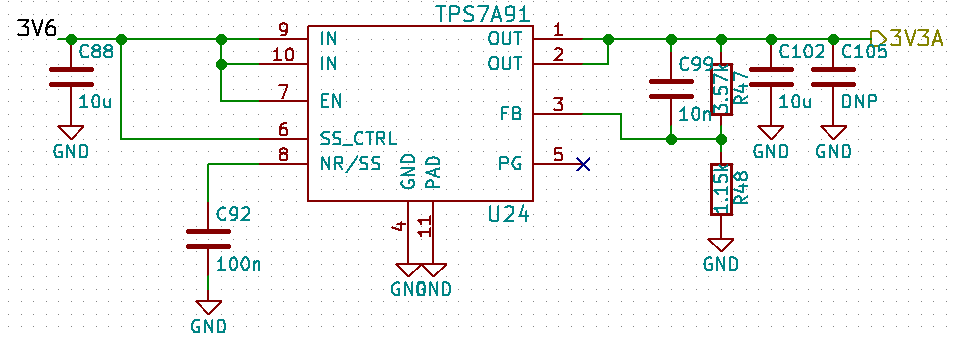
\includegraphics[width=0.75\textwidth]{data/linear-reg.png}
        \caption{A LDO regulator that takes as an input the voltage from one of the buck converters and
          whose output is directly used to drive the operation of one of the ICs elsewhere in the
          circuit.}
        \label{fig:linear-reg}
\end{figure}

The input voltage is connected to both IN pins with a bypass capacitor of 10 $\mu$F, which is the
minimum specified by the datasheet. It is additionally connected to the EN pin which activates the
LDO; the LDO is active for $V_{\text{EN}} \geq V_{\text{IH}}$ and disabled for
$V_{\text{EN}} \leq V_{\text{IL}}$ (connecting the same input to IN and EN will make
$V_{\text{EN}} = V_{\text{IH}}$, thus satisfying the first condition). The 2 resistors attached to
OUT and FB make a voltage divider that determines the output voltage of the linear regulator,
according to Equation~\ref{eq:linear-reg-vout}.

\begin{equation}
        R_1 = R_2\left(\frac{V_{\text{OUT}}}{V_{\text{REF}}}-1\right) \label{eq:linear-reg-vout}
\end{equation}

Where $V_{\text{REF}} = 0.8V$ Specifically, 1.15k and 3.57k are specified in the datasheet in order
to get an output voltage of 3.3V. SS\_CTRL is connected to IN instead of GND which increases the
soft-startup charging current to 100 $\mu$A from 6.2 $\mu$A and decreases the start-up time, which
is given by Equation~\ref{eq:linear-reg-startup-time}.

\begin{align}
  t_{\text{SS}} &= (V_{\text{REF}} \times C_{\text{NR/SS}}) /
                  I_{\text{NR/SS}} \label{eq:linear-reg-startup-time} \\
                &= 0.8V \times 100 \times 10^{-9} F/(100 \times 10^{-6} A) \\
                &= 0.8\text{ms}
\end{align}

An output capacitor of 10 $\mu$F is chosen which is the minimum specified by the
datasheet. Additionally, a feed-forward capacitor of 10nF is added between the OUT and FB pins to
improve the noise and PSRR performance of the voltage regulator. The value is recommended by the
datasheet. The $C_{\text{NR/SS}}$ capacitor of 100nF is used to create an output RC filter for
output noise and is also used to set the soft-start time. A value of between 10nF and 10$\mu$F is
recommended. PAD and GND should both be connected to ground, as indicated by the datasheet. PG
indicates whether the output voltage is in a usable state. Since we are not using it, it can be left
floating.

Another buck converter output feeds into the input of an ultra low LDO, with a dropout voltage of
40mV as shown in Figure~\ref{fig:ldo-ldo-connection}. R104 acts as a pull-up resistor, pulling the
voltage on EN high when PG is not driven. However, when PG is low, EN will be driven low. The bypass
pin is left open, although a 1$\mu$F capacitor could have been placed there to reduce output noise.

\begin{figure}[h]
        \centering
        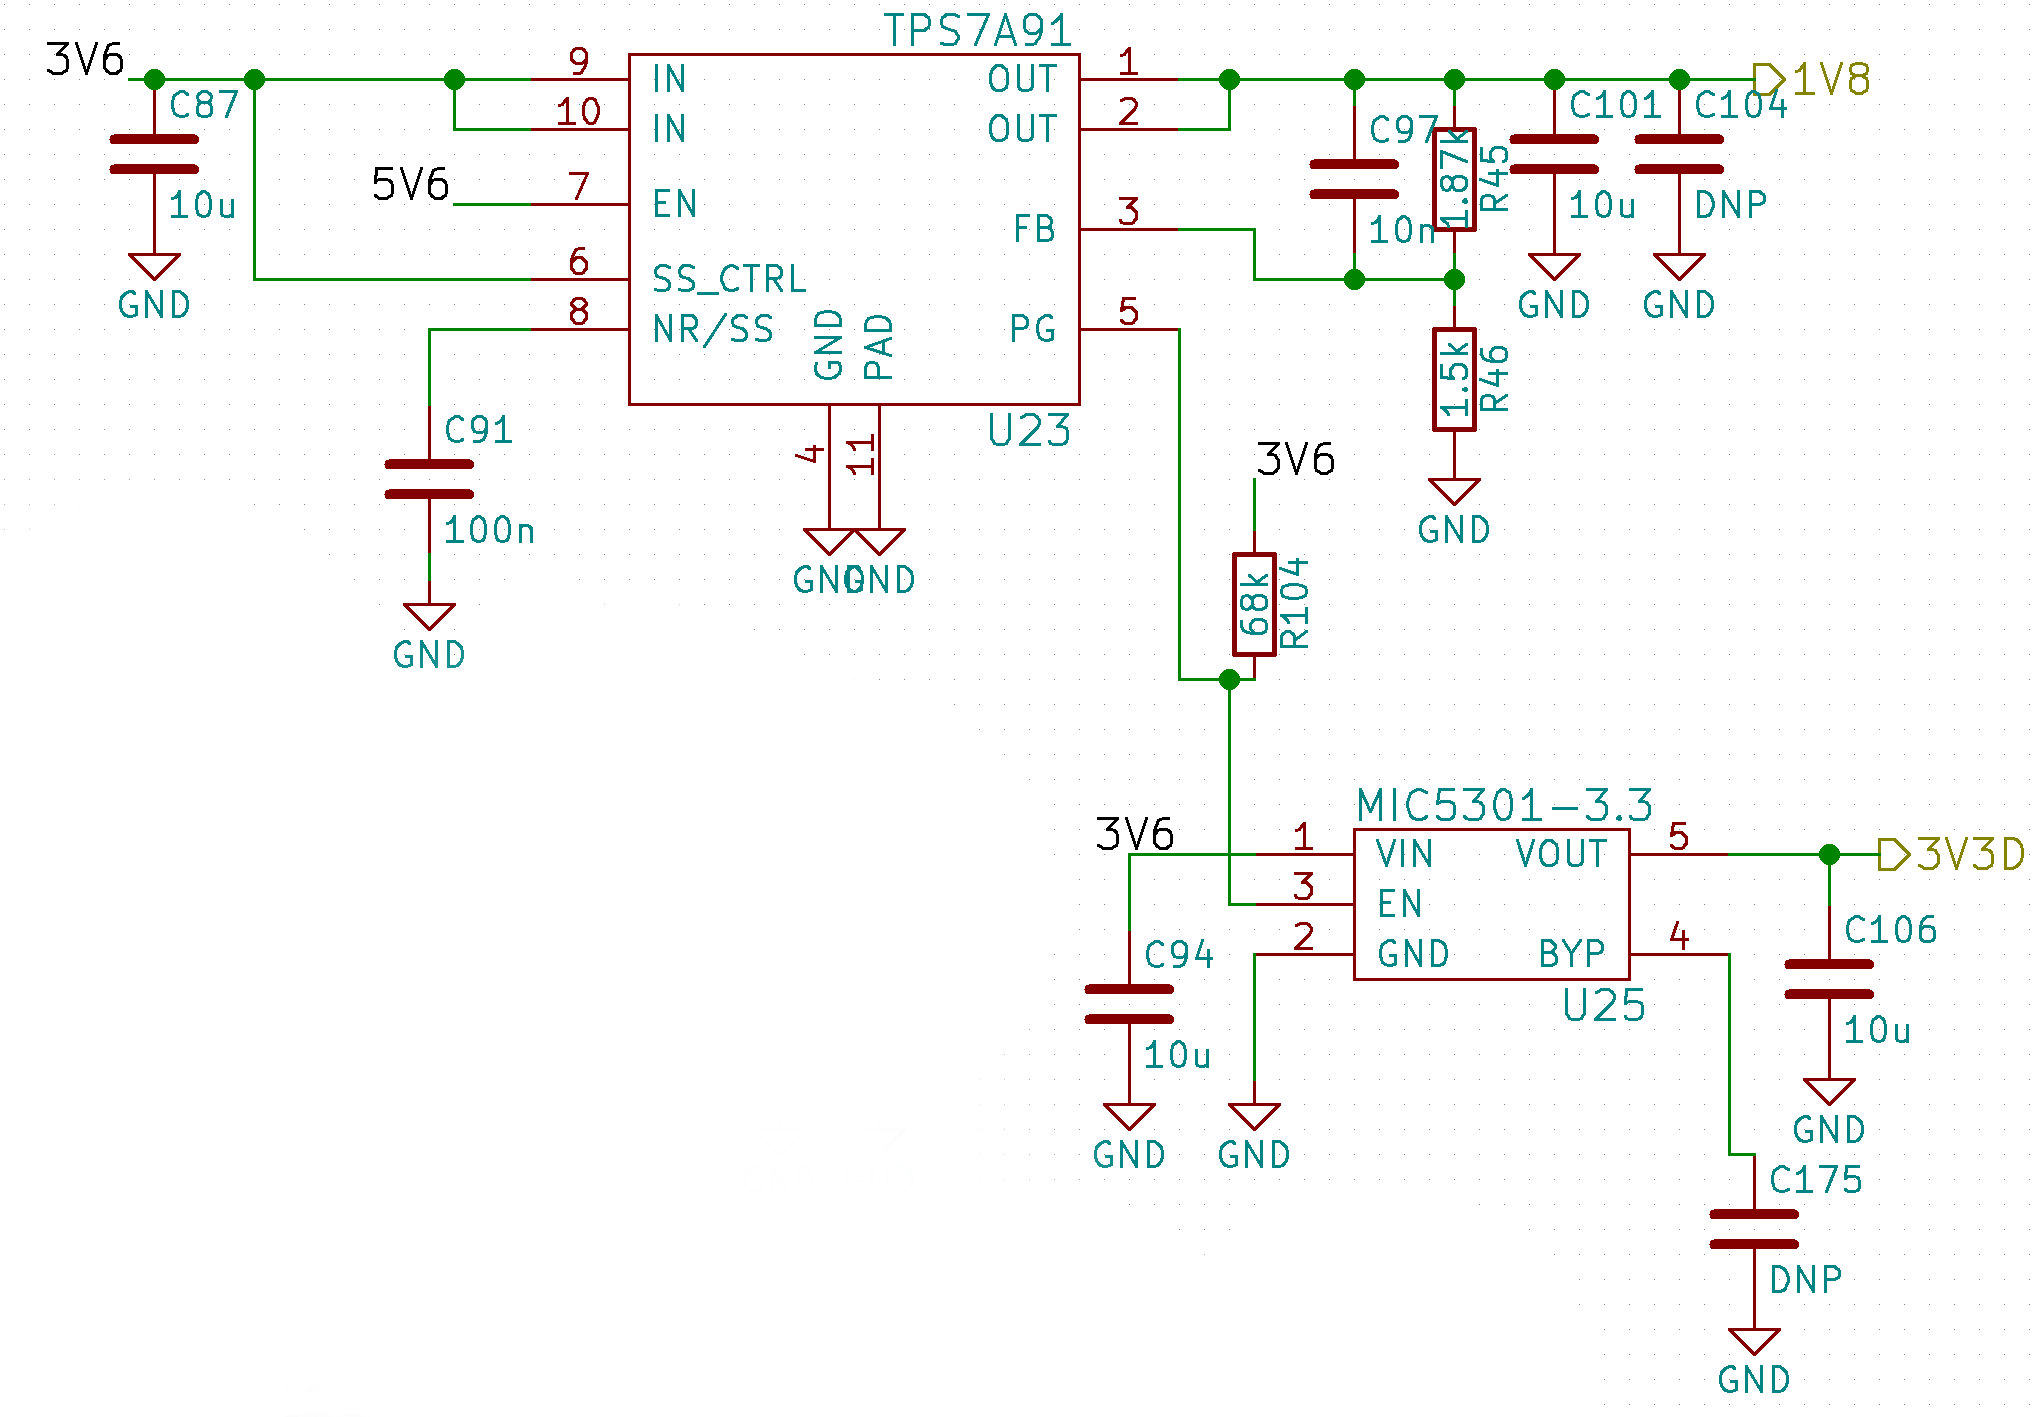
\includegraphics[width=0.9\textwidth]{data/ldo-ldo-connection.png}
        \caption{An ultra LDO regulator whose output feeds into an FPGA input. It uses the PG
          pin from another LDO regulator to alternately enable/disable it.}
        \label{fig:ldo-ldo-connection}
\end{figure}

Another output from a buck converter leads to a 3V output LDO regulator with a dropout voltage of
120mV shown in Figure~\ref{fig:lp5907}. All of the pin connections are evident.

\begin{figure}[h]
        \centering
        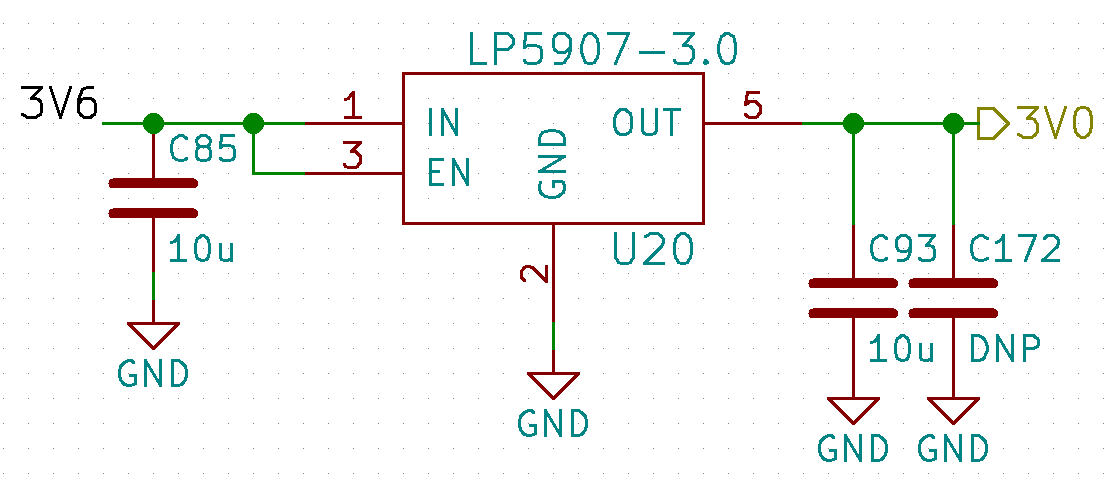
\includegraphics[width=0.75\textwidth]{data/lp5907.png}
        \caption{The LP5907 is a 3V LDO regulator with a dropout voltage of 120mV.}
        \label{fig:lp5907}
\end{figure}

The last component on the power sheet is an
\href{http://www.ti.com/lit/ds/symlink/lp2985.pdf}{LP2985} LDO regulator shown in
Figure~\ref{fig:lp2985}, that takes the 12V input voltage from the barrel jack and outputs
10V. ON/OFF is an active-low shutdown pin, so it is tied to $V_{\text{IN}}$. A 10nF capacitor is
tied to BYPASS to decrease the output noise.

\begin{figure}[h]
        \centering
        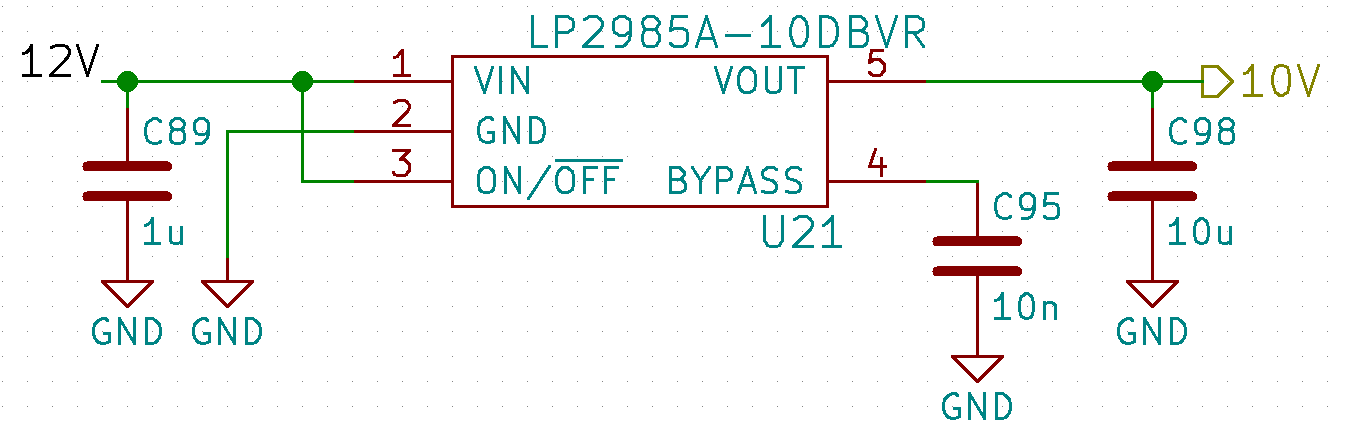
\includegraphics[width=0.9\textwidth]{data/lp2985.png}
        \caption{The LP2985 LDO regulator.}
        \label{fig:lp2985}
\end{figure}

\subsection{BOM}
\label{sec:power-bom}

\label{tab:power-schematic-components}
\begin{tabularx}{\textwidth}{c l l c X>{\raggedright\arraybackslash}X}
        \toprule
        \textbf{Designators} & \textbf{Description} & \textbf{MFN} & \textbf{QTY} & \textbf{Links} \\
        \midrule \endhead FB11 & barrel jack ferrite bead & 74279228600 & 1 &
        \href{https://katalog.we-online.de/pbs/datasheet/74279228600.pdf}{Datasheet},
        \href{https://www.digikey.com/product-detail/en/wurth-electronics-inc/74279228600/732-6119-1-ND/5050874}{Digi-Key}
        \\
        U18, U19 & buck converter & \hyperlink{sec:tps5420d}{TPS5420D} & 2 &
        \href{http://www.ti.com/lit/ds/symlink/tps5420.pdf}{Datasheet},
        \href{https://www.digikey.com/product-detail/en/texas-instruments/TPS5420DR/296-31984-1-ND/3505318}{Digi-Key}
        \\
        U21 & linear regulator & \hyperlink{sec:lp985a-10dbvr}{LP985A-10DBVR} & 1 &
        \href{https://www.ti.com/lit/ds/symlink/lp2985.pdf}{Datasheet},
        \href{https://www.digikey.com/product-detail/en/texas-instruments/LP2985A-10DBVR/296-24264-1-ND/2038549}{Digi-Key}
        \\
        \bottomrule
\end{tabularx}
%%% Local Variables:
%%% mode: latex
%%% TeX-master: "fmcw-radar"
%%% End:
